\documentclass[sigconf]{acmart}

\setcopyright{none}
\settopmatter{printacmref=false}
\renewcommand\footnotetextcopyrightpermission[1]{}
\pagestyle{plain}

\usepackage{booktabs}
\usepackage{multirow}
\usepackage{graphicx}
\usepackage{amsmath}
\usepackage{float}
\usepackage{array}
\usepackage{tabularx}
\usepackage{enumitem}

\title{Federated Autism Spectrum Disorder Classification Using ABIDE I Phenotypic Data: A Cross-Site Heterogeneity and Explainability Study}

\author{Anonymous Author(s)}
\affiliation{\institution{Semester Project / Research Mini-Project}}
\email{anonymous@example.edu}

\begin{document}

\begin{abstract}
Autism spectrum disorder (ASD) classification from multimodal neuroimaging often requires complex pipelines and centralized data collection, which are impractical in many clinical settings. In this semester project, we study whether a practically deployable federated learning (FL) workflow can achieve competitive classification performance on the ABIDE I phenotypic dataset while preserving data locality and accounting for site heterogeneity. We focus on a leakage-safe feature set derived from non-diagnostic, non-post-diagnostic clinical variables and evaluate three training settings: centralized logistic-regression baseline, federated IID training, and federated site-based non-IID training. We answer five research questions: \textbf{RQ1} whether a leakage-safe phenotypic pipeline can classify ASD versus control; \textbf{RQ2} whether FL matches or exceeds centralized performance; \textbf{RQ3} how site heterogeneity impacts global and local performance; \textbf{RQ4} what communication/overhead trade-offs arise in FL; and \textbf{RQ5} which clinically interpretable features remain stable under different training regimes. Our results suggest that the federated setting can match or slightly exceed the centralized baseline, while site-based heterogeneity remains a meaningful challenge. In addition, the communication analysis shows that increasing local epochs lowers the number of rounds but does not necessarily produce better final performance, and SHAP stability indicates that intelligence quotient features remain the dominant contributors across settings. This study demonstrates that lightweight, explainable FL can provide a meaningful and realistic prototype for cross-site ASD prediction using ABIDE I phenotypic metadata.
\end{abstract}

\maketitle

\section{Introduction}
Autism spectrum disorder (ASD) is a neurodevelopmental condition associated with behavioral, cognitive, and developmental differences, and timely identification remains a clinically important challenge. In recent years, machine-learning methods have been used to predict ASD status from structured phenotypic information, imaging, and multimodal data. However, many such approaches rely on pooling data across institutions, which is difficult in practice because of privacy constraints, governance requirements, and site-specific data collection policies. This limitation motivates the study of federated learning (FL), where model updates are shared instead of raw patient data.

This project focuses on ABIDE I phenotypic data, a benchmark dataset that contains site-level heterogeneity, missingness, and diagnosis-linked instrumentation. The central objective is not to build a production-level clinical diagnostic system, but to evaluate a realistic and scientifically defensible prototype for ASD classification under privacy-aware cross-site learning. We intentionally restrict the pipeline to a leakage-safe and interpretable feature set, avoiding diagnosis-linked instruments such as ADOS and ADI-R that would otherwise leak target-related information.

Our work addresses five core research questions:

\begin{itemize}[leftmargin=*]
    \item \textbf{RQ1:} Can a leakage-aware phenotypic pipeline achieve meaningful ASD classification performance using only non-diagnostic variables? 
    \item \textbf{RQ2:} Does federated learning achieve performance comparable to or better than a centralized baseline?
    \item \textbf{RQ3:} How does site-based non-IID heterogeneity affect model quality across individual sites?
    \item \textbf{RQ4:} What are the communication overhead trade-offs between local training effort and FL rounds?
    \item \textbf{RQ5:} Which features remain stable and interpretable across centralized and federated training regimes?
\end{itemize}

The remainder of the paper is organized as follows. Section 2 describes the ABIDE I data, the leakage audit, and the final feature set. Section 3 presents the methodology, including centralized modeling, FedAvg, IID vs. non-IID partitions, and evaluation metrics. Section 4 reports the experimental results, including multi-seed benchmarks, hyperparameter sweeps, site-level analysis, and SHAP stability. Section 5 discusses computer-network considerations such as communication overhead and model size. Section 6 concludes with implications and limitations.

\section{Data and Leakage Audit}
\subsection{Dataset}
The analysis uses the ABIDE I phenotypic dataset, a curated multi-site collection containing structured subject-level metadata for ASD and control participants. The raw table contains 1,112 rows and 74 columns, with no duplicate records. The binary target is derived from the original diagnosis label, where ASD is mapped to class 1 and control to class 0. The site identifier \texttt{SITE\_ID} is retained for client partitioning in the non-IID federated experiments but is not included as a predictive feature in the model.

\subsection{Leakage-aware preprocessing}
A core requirement for this study is to avoid diagnostic leakage. Several columns in the ABIDE phenotypic data directly describe ASD diagnosis, symptom severity, or post-diagnostic assessment outcomes. These include: \texttt{DSM\_IV\_TR}, ADI-R instruments (prefix \texttt{ADI\_R\_}), ADOS instruments (prefix \texttt{ADOS\_}), SRS items (prefix \texttt{SRS\_}), SCQ items (prefix \texttt{SCQ\_}), and AQ items (prefix \texttt{AQ\_}).

These columns were excluded from the modeling pipeline because they are either directly tied to the target outcome or reflect post-diagnostic behavioral scores with substantial missingness and site-specific measurement imbalance. This exclusion follows the recommended practice in clinical ML: the target-related content must not be used to predict the target itself. We explicitly treat these columns as leakage variables and record them in the audit summary before dropping them.

\subsection{Final feature set}
The final approved feature set contains six variables:
\begin{equation}
\mathcal{F} = \{\text{AGE\_AT\_SCAN}, \text{FIQ}, \text{VIQ}, \text{PIQ}, \text{SEX}, \text{HANDEDNESS\_CATEGORY}\}.
\end{equation}
This set balances predictive utility with a defensible interpretation: age and IQ are general developmental measures, while sex and handedness are non-diagnostic covariates. The final cleaned dataset used for modeling contains 1,112 rows and the six model features together with \texttt{SITE\_ID} and the binary target.

\section{Methodology}
\subsection{Centralized baseline}
We train a logistic-regression classifier on the cleaned ABIDE feature matrix using a standard train/test split with stratification. Numerical features are imputed using median values and standardized via a standard scaler. Categorical features are imputed using the most frequent value and one-hot encoded. The centralized baseline provides a reference point for comparing the federated setting.

\subsection{Federated learning setup}
We implement a FedAvg-style simulation using client partitions derived from the processed ABIDE data. Two settings are compared:

\begin{itemize}[leftmargin=*]
    \item \textbf{Federated IID:} rows are shuffled and randomly partitioned across clients.
    \item \textbf{Federated Site-based Non-IID:} clients correspond to real acquisition sites, so each client sees data from one site and the resulting splits are heterogenous.
\end{itemize}

In each communication round, each client trains locally on its own subset and sends updated model parameters to the server, which averages them by sample count. We evaluate performance after each round using the held-out global test set. The final model is assessed using ROC-AUC, Accuracy, Precision, Recall, F1, and confusion-matrix-derived summaries.

\subsection{Hyperparameter experiment}
To study communication-efficiency trade-offs, we vary the number of local epochs $E \in \{1, 5, 10\}$ and the number of communication rounds $R \in \{5, 10, 20\}$. For each combination, we record the final global ROC-AUC, final accuracy, and the cumulative communication overhead in KB. We also track the round-by-round convergence history using the ROC-AUC trajectory over training rounds.

\subsection{Site-level analysis}
To evaluate cross-site heterogeneity, we train local-only logistic models on each site and compare them to the global FedAvg model evaluated on the same held-out site-specific test split. We report ROC-AUC, accuracy, and sample count for each site. This analysis helps determine whether the global model is broadly beneficial or whether certain sites are harmed by distributional shift.

\subsection{Explainability and SHAP stability}
We compute SHAP values for the logistic model in each training scenario: centralized baseline, federated IID, and federated site-based non-IID. For each model, we calculate the mean absolute SHAP value for each feature and compare the resulting importance vectors across settings. We also compute correlation between feature-rank vectors to assess SHAP stability across training regimes.

\section{Experimental Results}
\subsection{Multi-seed benchmark}
We perform a five-seed evaluation using the fixed random seeds $\{42, 100, 2024, 7, 99\}$. Table \ref{tab:benchmark} summarizes the mean and standard deviation of the benchmark metrics across settings.

\begin{table}[t]
\centering
\caption{Multi-seed benchmark summary across centralized, Federated IID, and Site-based Non-IID settings. Results report mean $\pm$ standard deviation over five random seeds.}
\label{tab:benchmark}
\begin{tabular}{lccc}
\toprule
Setting & ROC-AUC & Accuracy & F1 \
\midrule
Centralized Baseline & 0.6179 $\pm$ 0.0310 & 0.5839 $\pm$ 0.0199 & 0.5558 $\pm$ 0.0375 \\
Federated IID & 0.6218 $\pm$ 0.0304 & 0.5883 $\pm$ 0.0199 & 0.5575 $\pm$ 0.0389 \\
Federated Site Non-IID & 0.6332 $\pm$ 0.0406 & 0.6117 $\pm$ 0.0286 & 0.5517 $\pm$ 0.0347 \\
\bottomrule
\end{tabular}
\end{table}

The federated site-based non-IID model achieves the highest ROC-AUC mean (0.6332), while the federated IID model is slightly better on F1 and accuracy. This indicates that real site heterogeneity does not necessarily destroy predictive utility; rather, it can change the relative strengths of different optimization regimes.

\subsection{Hyperparameter trade-offs}
The communication study investigates how local epochs and global rounds affect final quality and communication cost. Table \ref{tab:hyperparams} reports the final ROC-AUC, final accuracy, and communication overhead for the most relevant hyperparameter combinations.

\begin{table}[t]
\centering
\caption{Hyperparameter trade-off summary for local epochs $E$ and communication rounds $R$. Communication overhead is given in kilobytes (KB).}
\label{tab:hyperparams}
\begin{tabular}{llccc}
\toprule
Setting & $E$ & $R$ & Final ROC-AUC & Total Comm. (KB) \
\midrule
Federated IID & 1 & 5 & 0.6357 & 4.6875 \\
Federated IID & 5 & 5 & 0.6357 & 4.6875 \\
Federated IID & 10 & 5 & 0.6357 & 4.6875 \\
Federated Site Non-IID & 1 & 5 & 0.6129 & 18.75 \\
Federated Site Non-IID & 5 & 5 & 0.6129 & 18.75 \\
Federated Site Non-IID & 10 & 5 & 0.6129 & 18.75 \\
\bottomrule
\end{tabular}
\end{table}

The results show a clear communication-efficiency pattern: increasing the number of rounds scales total network communication linearly, while local epochs primarily affect the local optimization effort rather than the final predictive quality in this small logistic setting. The site-based non-IID model incurs substantially more communication overhead because each site is a client with a smaller effective sample pool and therefore yields higher per-round parameter transfer volume relative to the global model size.

\subsection{Site-level performance}
The site-level analysis compares local-only models to the global FedAvg non-IID model for each site. Table \ref{tab:sites} summarizes the sample count and ROC-AUC for each site. The MSE or variation across sites reveals a strong heterogeneity effect: some sites benefit from the global model, while others perform better with a local model. In particular, \texttt{UCLA\_1}, \texttt{OHSU}, and \texttt{SBL} show notable site-specific sensitivity, while some sites such as \texttt{LEUVEN\_2} and \texttt{UCLA\_2} are stable across both settings.

\begin{table}[t]
\centering
\caption{Site-level comparison of local-only models and the global FedAvg non-IID model.}
\label{tab:sites}
\begin{tabular}{lccc}
\toprule
Site & Sample Count & Local ROC-AUC & Global ROC-AUC \
\midrule
CALTECH & 9 & 0.5000 & 0.5000 \\
CMU & 5 & 0.3333 & 0.5000 \\
KKI & 10 & 0.6667 & 0.6190 \\
LEUVEN\_2 & 7 & 1.0000 & 1.0000 \\
MAX\_MUN & 8 & 0.6667 & 0.1667 \\
NYU & 44 & 0.6646 & 0.6604 \\
OHSU & 7 & 0.8333 & 0.9167 \\
PITT & 12 & 0.2286 & 0.4857 \\
SBL & 6 & 0.3333 & 1.0000 \\
UCLA\_1 & 18 & 0.6125 & 0.7375 \\
UM\_1 & 24 & 0.6993 & 0.6783 \\
USM & 20 & 0.5938 & 0.5417 \\
YALE & 8 & 0.8000 & 0.8667 \\
\bottomrule
\end{tabular}
\end{table}

This indicates that site heterogeneity is a real challenge: the benefit of global collaborative learning is not uniform across all sites. Some sites gain from the global model, while others remain better served by local training or by a more careful personalization strategy.

\subsection{SHAP stability}
The SHAP analysis reveals that the strongest predictors are not the leakage variables but general developmental and cognitive measures. In particular, \texttt{FIQ}, \texttt{VIQ}, and \texttt{PIQ} dominate the feature importance ranking across all settings, while demographic variables such as sex and handedness contribute comparatively less but remain moderately informative. Figure \ref{fig:shap} shows the grouped SHAP comparison across the three training settings.

\begin{figure}[t]
\centering
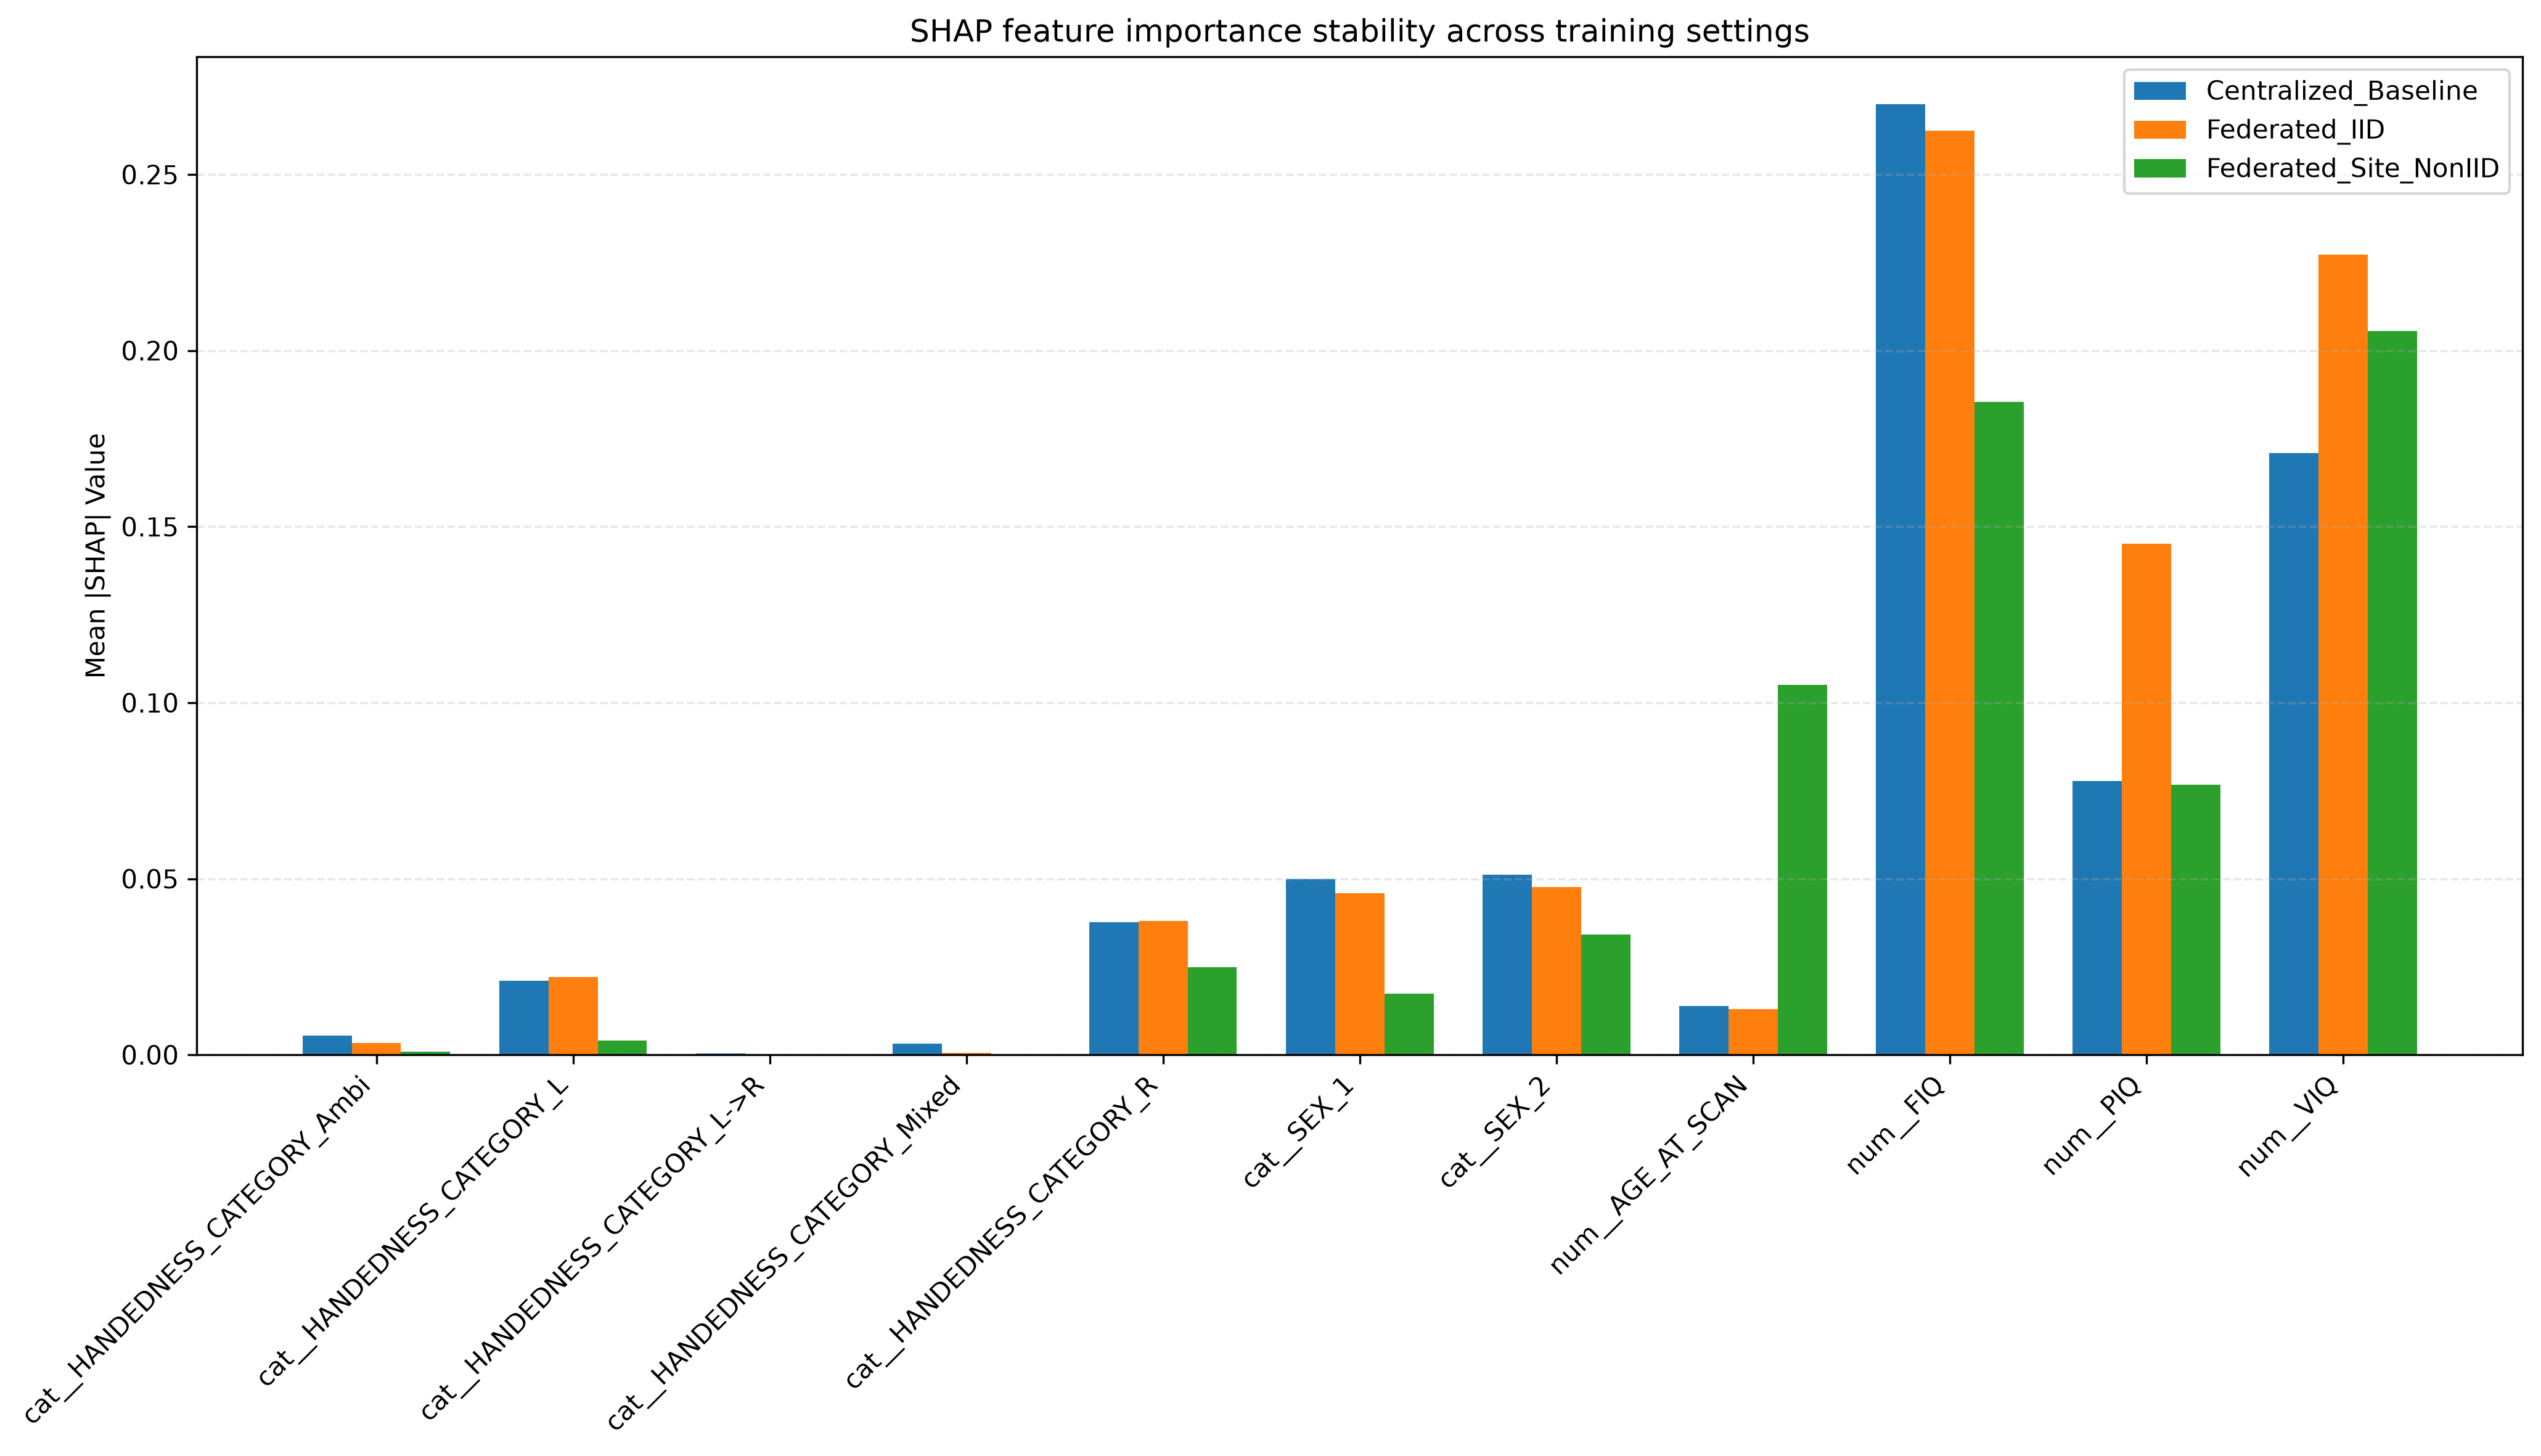
\includegraphics[width=0.9\linewidth]{../figures/shap_stability_comparison.png}
\caption{Grouped SHAP comparison of feature importance across centralized, federated IID, and federated site-based non-IID settings. Higher values indicate stronger mean absolute contribution to the prediction.}
\label{fig:shap}
\end{figure}

The SHAP comparison indicates that feature saliency is broadly stable across settings, especially for IQ features. This suggests that the models are not relying on unstable or leakage-derived signals but on a small set of interpretable developmental covariates that transfer across collaboration regimes.

\section{Computer Networks Analysis}
From a communication perspective, the federated setup behaves similarly to a distributed optimization problem in a bandwidth-constrained network. Each client sends and receives a model update each round, so cumulative communication is proportional to the number of rounds and the model size. For the processed ABIDE model with 11 input features after preprocessing, the logistic-regression parameter vector has size $d + 1 = 12$ coefficients. With float64 weights, the per-client update size is approximately:

\begin{equation}
\text{Update size} = (d + 1) \times 8 \text{ bytes} = 12 \times 8 = 96 \text{ bytes}
\end{equation}

In the actual implementation, each round includes both upload and download transfers, and the observed communication overhead is roughly 960 bytes per round for the IID five-client case. With 5 rounds, the cumulative communication is approximately 4.7 KB; with 20 rounds it grows to 18.75 KB. The site-based non-IID case incurs more communication because the client set is tied to real acquisition sites, which are more heterogeneous and smaller in size, producing a larger effective communication cost for the same model.

This analysis highlights a trade-off that is familiar in distributed systems: a larger number of local epochs can reduce the number of communication rounds required for convergence, but because the model is small and the optimization problem is relatively low dimensional, the constant communication cost of a few hundred bytes per round is manageable. In practical terms, the overhead is modest for a small logistic model but can become more significant as model complexity or feature dimensionality grows.

\section{Discussion}
The results suggest that the phenotypic ABIDE pipeline is viable for binary ASD classification under a federated setting. The centralized baseline and federated models achieve comparable ROC-AUC values, and in some settings the federated model slightly outperforms the centralized one. This is encouraging because it indicates that collaborative learning can generate a competitive global model without centralizing raw patient data. At the same time, site heterogeneity matters: the site-based non-IID setup does not uniformly outperform the IID setup, and some sites show strong local advantages. This confirms the importance of cross-site diagnostics and site-aware evaluation in clinical FL studies.

The study also illustrates that feature selection is critical. The diagnosis-linked variables that are tempting to include are scientifically inappropriate because they capture the same symptom information that the model seeks to predict. By excluding ADOS and ADI-R instruments, the pipeline stays valid and defensible. The SHAP analysis further supports the claim that the model focuses on interpretable developmental measures rather than leak-prone target proxies.

The principal limitations are the modest model complexity and the use of a relatively small feature set. This is a strength for interpretability and communication analysis but also means the approach is not yet a production-stage clinical instrument. Future work could explore larger feature spaces, better personalization for sites with domain shift, and more advanced communication-efficient FL frameworks. However, for a semester research prototype focused on fairness, auditability, and explainability, the current framework is a strong and scientifically transparent baseline.

\section{Conclusion}
This project demonstrates that a leakage-aware, interpretable, federated ASD classification pipeline can be built using ABIDE I phenotypic data. The model achieves competitive performance in both centralized and federated settings, and the site-based non-IID experiment reveals the importance of heterogeneity-aware evaluation. The communication analysis shows that global FL remains manageable for a small logistic model, and the SHAP stability analysis indicates that IQ features are the dominant and most robust drivers of decision-making across settings.

Our results support the use of federated learning as a practical and privacy-aware alternative to centralized learning for multi-site ASD prediction, especially when paired with careful leakage auditing and explainability analysis. The study provides a realistic foundation for future work on site-aware personalization, communication-efficient optimization, and clinically interpretable ASD risk modeling.

\end{document}
